\documentclass[twoside]{book}

% Packages required by doxygen
\usepackage{fixltx2e}
\usepackage{calc}
\usepackage{doxygen}
\usepackage[export]{adjustbox} % also loads graphicx
\usepackage{graphicx}
\usepackage[utf8]{inputenc}
\usepackage{makeidx}
\usepackage{multicol}
\usepackage{multirow}
\PassOptionsToPackage{warn}{textcomp}
\usepackage{textcomp}
\usepackage[nointegrals]{wasysym}
\usepackage[table]{xcolor}

% Font selection
\usepackage[T1]{fontenc}
\usepackage[scaled=.90]{helvet}
\usepackage{courier}
\usepackage{amssymb}
\usepackage{sectsty}
\renewcommand{\familydefault}{\sfdefault}
\allsectionsfont{%
  \fontseries{bc}\selectfont%
  \color{darkgray}%
}
\renewcommand{\DoxyLabelFont}{%
  \fontseries{bc}\selectfont%
  \color{darkgray}%
}
\newcommand{\+}{\discretionary{\mbox{\scriptsize$\hookleftarrow$}}{}{}}

% Page & text layout
\usepackage{geometry}
\geometry{%
  a4paper,%
  top=2.5cm,%
  bottom=2.5cm,%
  left=2.5cm,%
  right=2.5cm%
}
\tolerance=750
\hfuzz=15pt
\hbadness=750
\setlength{\emergencystretch}{15pt}
\setlength{\parindent}{0cm}
\setlength{\parskip}{3ex plus 2ex minus 2ex}
\makeatletter
\renewcommand{\paragraph}{%
  \@startsection{paragraph}{4}{0ex}{-1.0ex}{1.0ex}{%
    \normalfont\normalsize\bfseries\SS@parafont%
  }%
}
\renewcommand{\subparagraph}{%
  \@startsection{subparagraph}{5}{0ex}{-1.0ex}{1.0ex}{%
    \normalfont\normalsize\bfseries\SS@subparafont%
  }%
}
\makeatother

% Headers & footers
\usepackage{fancyhdr}
\pagestyle{fancyplain}
\fancyhead[LE]{\fancyplain{}{\bfseries\thepage}}
\fancyhead[CE]{\fancyplain{}{}}
\fancyhead[RE]{\fancyplain{}{\bfseries\leftmark}}
\fancyhead[LO]{\fancyplain{}{\bfseries\rightmark}}
\fancyhead[CO]{\fancyplain{}{}}
\fancyhead[RO]{\fancyplain{}{\bfseries\thepage}}
\fancyfoot[LE]{\fancyplain{}{}}
\fancyfoot[CE]{\fancyplain{}{}}
\fancyfoot[RE]{\fancyplain{}{\bfseries\scriptsize Generated by Doxygen }}
\fancyfoot[LO]{\fancyplain{}{\bfseries\scriptsize Generated by Doxygen }}
\fancyfoot[CO]{\fancyplain{}{}}
\fancyfoot[RO]{\fancyplain{}{}}
\renewcommand{\footrulewidth}{0.4pt}
\renewcommand{\chaptermark}[1]{%
  \markboth{#1}{}%
}
\renewcommand{\sectionmark}[1]{%
  \markright{\thesection\ #1}%
}

% Indices & bibliography
\usepackage{natbib}
\usepackage[titles]{tocloft}
\setcounter{tocdepth}{3}
\setcounter{secnumdepth}{5}
\makeindex

% Hyperlinks (required, but should be loaded last)
\usepackage{ifpdf}
\ifpdf
  \usepackage[pdftex,pagebackref=true]{hyperref}
\else
  \usepackage[ps2pdf,pagebackref=true]{hyperref}
\fi
\hypersetup{%
  colorlinks=true,%
  linkcolor=blue,%
  citecolor=blue,%
  unicode%
}

% Custom commands
\newcommand{\clearemptydoublepage}{%
  \newpage{\pagestyle{empty}\cleardoublepage}%
}

\usepackage{caption}
\captionsetup{labelsep=space,justification=centering,font={bf},singlelinecheck=off,skip=4pt,position=top}

%===== C O N T E N T S =====

\begin{document}

% Titlepage & ToC
\hypersetup{pageanchor=false,
             bookmarksnumbered=true,
             pdfencoding=unicode
            }
\pagenumbering{alph}
\begin{titlepage}
\vspace*{7cm}
\begin{center}%
{\Large Projekt\+P\+OS }\\
\vspace*{1cm}
{\large Generated by Doxygen 1.8.13}\\
\end{center}
\end{titlepage}
\clearemptydoublepage
\pagenumbering{roman}
\tableofcontents
\clearemptydoublepage
\pagenumbering{arabic}
\hypersetup{pageanchor=true}

%--- Begin generated contents ---
\chapter{Namespace Index}
\section{Packages}
Here are the packages with brief descriptions (if available)\+:\begin{DoxyCompactList}
\item\contentsline{section}{\hyperlink{namespace_projekt_p_o_s}{Projekt\+P\+OS} }{\pageref{namespace_projekt_p_o_s}}{}
\end{DoxyCompactList}

\chapter{Hierarchical Index}
\section{Class Hierarchy}
This inheritance list is sorted roughly, but not completely, alphabetically\+:\begin{DoxyCompactList}
\item Application\begin{DoxyCompactList}
\item \contentsline{section}{Projekt\+P\+O\+S.\+App}{\pageref{class_projekt_p_o_s_1_1_app}}{}
\end{DoxyCompactList}
\item \contentsline{section}{Projekt\+P\+O\+S.\+List\+Extensions}{\pageref{class_projekt_p_o_s_1_1_list_extensions}}{}
\item \contentsline{section}{Projekt\+P\+O\+S.\+Postac}{\pageref{class_projekt_p_o_s_1_1_postac}}{}
\item \contentsline{section}{Projekt\+P\+O\+S.\+Utils}{\pageref{class_projekt_p_o_s_1_1_utils}}{}
\item Window\begin{DoxyCompactList}
\item \contentsline{section}{Projekt\+P\+O\+S.\+Main\+Window}{\pageref{class_projekt_p_o_s_1_1_main_window}}{}
\end{DoxyCompactList}
\end{DoxyCompactList}

\chapter{Class Index}
\section{Class List}
Here are the classes, structs, unions and interfaces with brief descriptions\+:\begin{DoxyCompactList}
\item\contentsline{section}{\hyperlink{class_projekt_p_o_s_1_1_app}{Projekt\+P\+O\+S.\+App} \\*Interaction logic for App.\+xaml }{\pageref{class_projekt_p_o_s_1_1_app}}{}
\item\contentsline{section}{\hyperlink{class_projekt_p_o_s_1_1_list_extensions}{Projekt\+P\+O\+S.\+List\+Extensions} \\*List extensions. }{\pageref{class_projekt_p_o_s_1_1_list_extensions}}{}
\item\contentsline{section}{\hyperlink{class_projekt_p_o_s_1_1_main_window}{Projekt\+P\+O\+S.\+Main\+Window} \\*Interaction logic for Main\+Window.\+xaml }{\pageref{class_projekt_p_o_s_1_1_main_window}}{}
\item\contentsline{section}{\hyperlink{class_projekt_p_o_s_1_1_postac}{Projekt\+P\+O\+S.\+Postac} \\*This class contains three fields\+: int Id, string I\+M\+IE, string N\+A\+Z\+W\+I\+S\+KO. }{\pageref{class_projekt_p_o_s_1_1_postac}}{}
\item\contentsline{section}{\hyperlink{class_projekt_p_o_s_1_1_utils}{Projekt\+P\+O\+S.\+Utils} \\*This is a public class that contains Wczytaj\+Dane method. }{\pageref{class_projekt_p_o_s_1_1_utils}}{}
\end{DoxyCompactList}

\chapter{Namespace Documentation}
\hypertarget{namespace_projekt_p_o_s}{}\section{Projekt\+P\+OS Namespace Reference}
\label{namespace_projekt_p_o_s}\index{Projekt\+P\+OS@{Projekt\+P\+OS}}
\subsection*{Classes}
\begin{DoxyCompactItemize}
\item 
class \hyperlink{class_projekt_p_o_s_1_1_app}{App}
\begin{DoxyCompactList}\small\item\em Interaction logic for App.\+xaml \end{DoxyCompactList}\item 
class \hyperlink{class_projekt_p_o_s_1_1_list_extensions}{List\+Extensions}
\begin{DoxyCompactList}\small\item\em List extensions. \end{DoxyCompactList}\item 
class \hyperlink{class_projekt_p_o_s_1_1_main_window}{Main\+Window}
\begin{DoxyCompactList}\small\item\em Interaction logic for Main\+Window.\+xaml \end{DoxyCompactList}\item 
class \hyperlink{class_projekt_p_o_s_1_1_postac}{Postac}
\begin{DoxyCompactList}\small\item\em This class contains three fields\+: int Id, string I\+M\+IE, string N\+A\+Z\+W\+I\+S\+KO. \end{DoxyCompactList}\item 
class \hyperlink{class_projekt_p_o_s_1_1_utils}{Utils}
\begin{DoxyCompactList}\small\item\em This is a public class that contains Wczytaj\+Dane method. \end{DoxyCompactList}\end{DoxyCompactItemize}

\chapter{Class Documentation}
\hypertarget{class_projekt_p_o_s_1_1_app}{}\section{Projekt\+P\+O\+S.\+App Class Reference}
\label{class_projekt_p_o_s_1_1_app}\index{Projekt\+P\+O\+S.\+App@{Projekt\+P\+O\+S.\+App}}


Interaction logic for App.\+xaml  


Inheritance diagram for Projekt\+P\+O\+S.\+App\+:\begin{figure}[H]
\begin{center}
\leavevmode
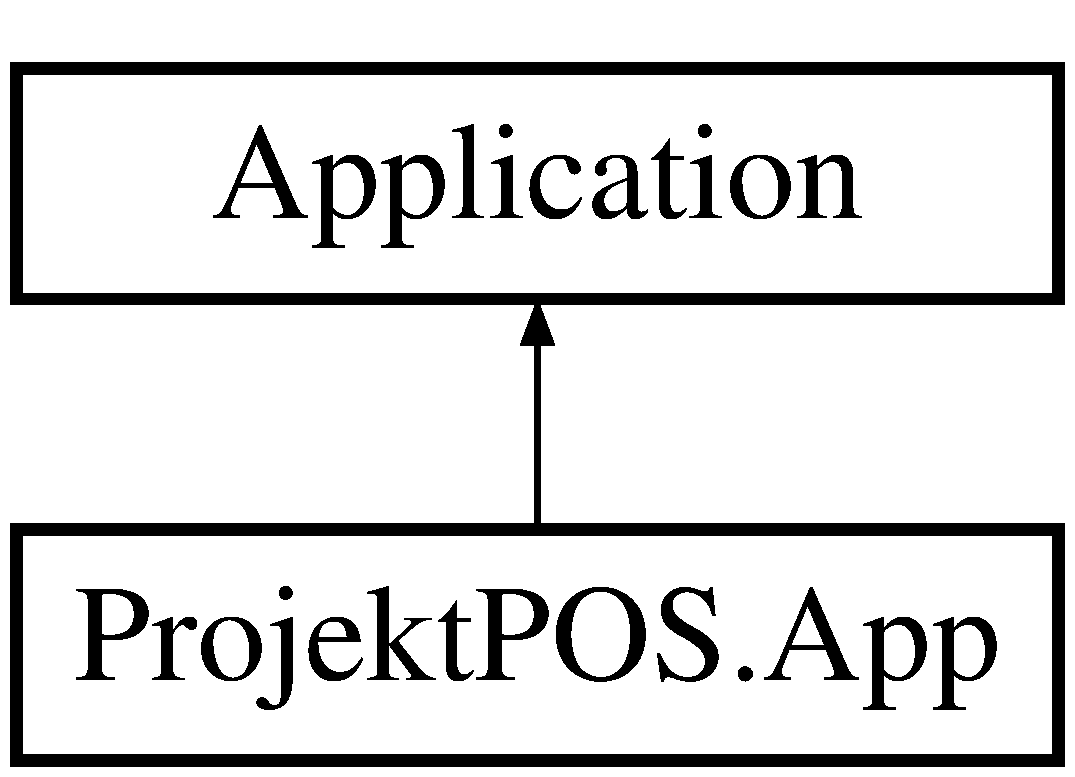
\includegraphics[height=2.000000cm]{class_projekt_p_o_s_1_1_app}
\end{center}
\end{figure}


\subsection{Detailed Description}
Interaction logic for App.\+xaml 



The documentation for this class was generated from the following file\+:\begin{DoxyCompactItemize}
\item 
D\+:/\+Przebudzenie Mocy/\+S\+Q\+Lite/\+O\+P\+T\+O\+P\+O\+S R\+E\+Pwc/trunk/\+Projekt\+P\+O\+S/\+Projekt\+P\+O\+S/App.\+xaml.\+cs\end{DoxyCompactItemize}

\hypertarget{class_projekt_p_o_s_1_1_list_extensions}{}\section{Projekt\+P\+O\+S.\+List\+Extensions Class Reference}
\label{class_projekt_p_o_s_1_1_list_extensions}\index{Projekt\+P\+O\+S.\+List\+Extensions@{Projekt\+P\+O\+S.\+List\+Extensions}}


List extensions.  


\subsection*{Static Public Member Functions}
\begin{DoxyCompactItemize}
\item 
static int \hyperlink{class_projekt_p_o_s_1_1_list_extensions_aaec21e8ac3689f1e2b9ebccf8eadd64a}{Max\+Id} (this List$<$ \hyperlink{class_projekt_p_o_s_1_1_postac}{Postac} $>$ postacie)
\begin{DoxyCompactList}\small\item\em This method is signed to list that contains \hyperlink{class_projekt_p_o_s_1_1_postac}{Postac} class objects. \end{DoxyCompactList}\end{DoxyCompactItemize}


\subsection{Detailed Description}
List extensions. 



\subsection{Member Function Documentation}
\mbox{\Hypertarget{class_projekt_p_o_s_1_1_list_extensions_aaec21e8ac3689f1e2b9ebccf8eadd64a}\label{class_projekt_p_o_s_1_1_list_extensions_aaec21e8ac3689f1e2b9ebccf8eadd64a}} 
\index{Projekt\+P\+O\+S\+::\+List\+Extensions@{Projekt\+P\+O\+S\+::\+List\+Extensions}!Max\+Id@{Max\+Id}}
\index{Max\+Id@{Max\+Id}!Projekt\+P\+O\+S\+::\+List\+Extensions@{Projekt\+P\+O\+S\+::\+List\+Extensions}}
\subsubsection{\texorpdfstring{Max\+Id()}{MaxId()}}
{\footnotesize\ttfamily static int Projekt\+P\+O\+S.\+List\+Extensions.\+Max\+Id (\begin{DoxyParamCaption}\item[{this List$<$ \hyperlink{class_projekt_p_o_s_1_1_postac}{Postac} $>$}]{postacie }\end{DoxyParamCaption})\hspace{0.3cm}{\ttfamily [static]}}



This method is signed to list that contains \hyperlink{class_projekt_p_o_s_1_1_postac}{Postac} class objects. 



The documentation for this class was generated from the following file\+:\begin{DoxyCompactItemize}
\item 
D\+:/\+Przebudzenie Mocy/\+S\+Q\+Lite/\+O\+P\+T\+O\+P\+O\+S R\+E\+Pwc/trunk/\+Projekt\+P\+O\+S/\+Projekt\+P\+O\+S/List\+Extensions.\+cs\end{DoxyCompactItemize}

\hypertarget{class_projekt_p_o_s_1_1_main_window}{}\section{Projekt\+P\+O\+S.\+Main\+Window Class Reference}
\label{class_projekt_p_o_s_1_1_main_window}\index{Projekt\+P\+O\+S.\+Main\+Window@{Projekt\+P\+O\+S.\+Main\+Window}}


Interaction logic for Main\+Window.\+xaml  


Inheritance diagram for Projekt\+P\+O\+S.\+Main\+Window\+:\begin{figure}[H]
\begin{center}
\leavevmode
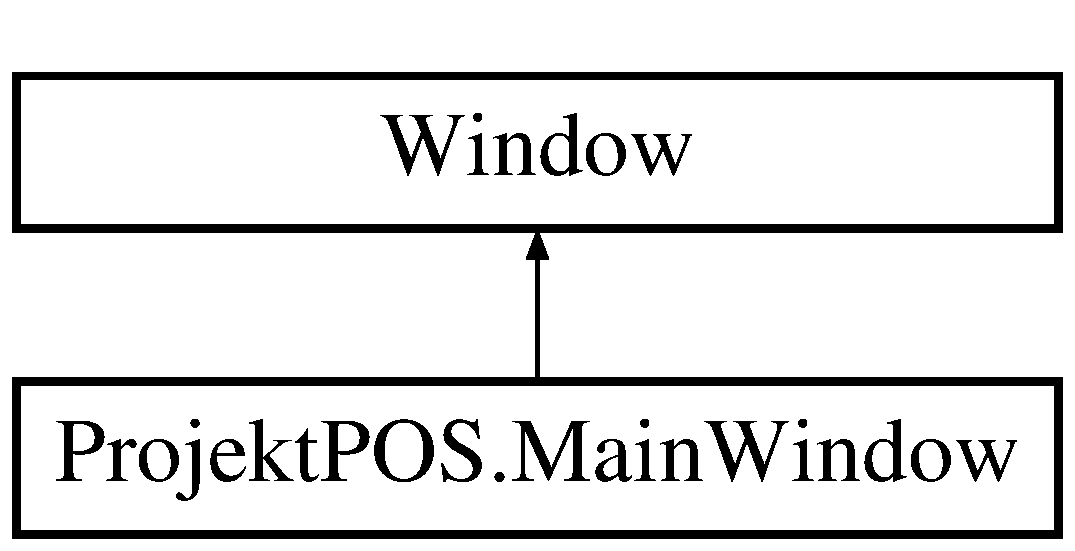
\includegraphics[height=2.000000cm]{class_projekt_p_o_s_1_1_main_window}
\end{center}
\end{figure}
\subsection*{Public Member Functions}
\begin{DoxyCompactItemize}
\item 
\hyperlink{class_projekt_p_o_s_1_1_main_window_accd74500e15ba53e22f8c803e78e3e65}{Main\+Window} ()
\begin{DoxyCompactList}\small\item\em This is the Main Window. \end{DoxyCompactList}\end{DoxyCompactItemize}
\subsection*{Private Member Functions}
\begin{DoxyCompactItemize}
\item 
void \hyperlink{class_projekt_p_o_s_1_1_main_window_a1c820b42a3dc4d0baa35192573a3248d}{Inicjalizacja\+Danych} ()
\begin{DoxyCompactList}\small\item\em This method adds \hyperlink{class_projekt_p_o_s_1_1_postac}{Postac} class objects to the list\+Box. It uses Wczytaj\+Dane method. \end{DoxyCompactList}\item 
\mbox{\Hypertarget{class_projekt_p_o_s_1_1_main_window_af6467cccd96f7169e8a84094d0017c1b}\label{class_projekt_p_o_s_1_1_main_window_af6467cccd96f7169e8a84094d0017c1b}} 
void {\bfseries imie\+Box\+\_\+\+Text\+Changed} (object sender, Text\+Changed\+Event\+Args e)
\item 
void \hyperlink{class_projekt_p_o_s_1_1_main_window_a98a2b1c31cf135c85a3c8bc12a9879ad}{button\+\_\+\+Click} (object sender, Routed\+Event\+Args e)
\begin{DoxyCompactList}\small\item\em Button \char`\"{}\+Baza\char`\"{} This method refreshes list\+Box. \end{DoxyCompactList}\item 
void \hyperlink{class_projekt_p_o_s_1_1_main_window_a955fd8db95c7491807d1262fdb15a115}{button2\+\_\+\+Click} (object sender, Routed\+Event\+Args e)
\begin{DoxyCompactList}\small\item\em Button \char`\"{}\+Aktualizuj\char`\"{} This method updates selected object from the list\+Box in the data base. \end{DoxyCompactList}\item 
void \hyperlink{class_projekt_p_o_s_1_1_main_window_a5b2c07df737c6583f39ba146500523eb}{list\+Box\+\_\+\+Selection\+Changed} (object sender, Selection\+Changed\+Event\+Args e)
\begin{DoxyCompactList}\small\item\em This method \end{DoxyCompactList}\item 
void \hyperlink{class_projekt_p_o_s_1_1_main_window_a0f8ea018177f274247e6d4601fb9e76e}{button\+Add\+\_\+\+Click} (object sender, Routed\+Event\+Args e)
\begin{DoxyCompactList}\small\item\em Button \char`\"{}\+Dodaj\char`\"{} This method adds \hyperlink{class_projekt_p_o_s_1_1_postac}{Postac} calss object to the data base. It uses text\+Boxs\+: imie\+Box, nazwisko\+Box. \end{DoxyCompactList}\item 
void \hyperlink{class_projekt_p_o_s_1_1_main_window_ac955d8aa2cc3dceeafa88d532c69a5e3}{button\+Delete\+\_\+\+Click} (object sender, Routed\+Event\+Args e)
\begin{DoxyCompactList}\small\item\em Button \char`\"{}\+Usuń\char`\"{} This method deletes \hyperlink{class_projekt_p_o_s_1_1_postac}{Postac} class object form the data base. \end{DoxyCompactList}\item 
void \hyperlink{class_projekt_p_o_s_1_1_main_window_a86639632a4f0c369581fba5be73a211f}{button1\+\_\+\+Click} (object sender, Routed\+Event\+Args e)
\begin{DoxyCompactList}\small\item\em Button \char`\"{}\+Zamknij\char`\"{} This method closes the \hyperlink{class_projekt_p_o_s_1_1_main_window}{Main\+Window}. \end{DoxyCompactList}\end{DoxyCompactItemize}
\subsection*{Private Attributes}
\begin{DoxyCompactItemize}
\item 
S\+Q\+Lite\+Connection \hyperlink{class_projekt_p_o_s_1_1_main_window_a9b68fbebcc348b5a1d0a0370d1180ba6}{\+\_\+polaczenie} = new S\+Q\+Lite\+Connection(\char`\"{}Data Source=baza.\+db\char`\"{})
\begin{DoxyCompactList}\small\item\em This field connects to data base file or creats new one. \end{DoxyCompactList}\item 
List$<$ \hyperlink{class_projekt_p_o_s_1_1_postac}{Postac} $>$ \hyperlink{class_projekt_p_o_s_1_1_main_window_abe462d9c2e721c3476d858fb870fa4b4}{lista\+Postaci} = new List$<$\hyperlink{class_projekt_p_o_s_1_1_postac}{Postac}$>$()
\begin{DoxyCompactList}\small\item\em This list contains \hyperlink{class_projekt_p_o_s_1_1_postac}{Postac} class objects. \end{DoxyCompactList}\item 
\hyperlink{class_projekt_p_o_s_1_1_postac}{Postac} \hyperlink{class_projekt_p_o_s_1_1_main_window_ad0cd50357b42ca42fed4b16ba859c645}{wybrana\+Postac} = null
\begin{DoxyCompactList}\small\item\em This field contains selected item from the list\+Box \end{DoxyCompactList}\end{DoxyCompactItemize}


\subsection{Detailed Description}
Interaction logic for Main\+Window.\+xaml 



\subsection{Constructor \& Destructor Documentation}
\mbox{\Hypertarget{class_projekt_p_o_s_1_1_main_window_accd74500e15ba53e22f8c803e78e3e65}\label{class_projekt_p_o_s_1_1_main_window_accd74500e15ba53e22f8c803e78e3e65}} 
\index{Projekt\+P\+O\+S\+::\+Main\+Window@{Projekt\+P\+O\+S\+::\+Main\+Window}!Main\+Window@{Main\+Window}}
\index{Main\+Window@{Main\+Window}!Projekt\+P\+O\+S\+::\+Main\+Window@{Projekt\+P\+O\+S\+::\+Main\+Window}}
\subsubsection{\texorpdfstring{Main\+Window()}{MainWindow()}}
{\footnotesize\ttfamily Projekt\+P\+O\+S.\+Main\+Window.\+Main\+Window (\begin{DoxyParamCaption}{ }\end{DoxyParamCaption})}



This is the Main Window. 



\subsection{Member Function Documentation}
\mbox{\Hypertarget{class_projekt_p_o_s_1_1_main_window_a86639632a4f0c369581fba5be73a211f}\label{class_projekt_p_o_s_1_1_main_window_a86639632a4f0c369581fba5be73a211f}} 
\index{Projekt\+P\+O\+S\+::\+Main\+Window@{Projekt\+P\+O\+S\+::\+Main\+Window}!button1\+\_\+\+Click@{button1\+\_\+\+Click}}
\index{button1\+\_\+\+Click@{button1\+\_\+\+Click}!Projekt\+P\+O\+S\+::\+Main\+Window@{Projekt\+P\+O\+S\+::\+Main\+Window}}
\subsubsection{\texorpdfstring{button1\+\_\+\+Click()}{button1\_Click()}}
{\footnotesize\ttfamily void Projekt\+P\+O\+S.\+Main\+Window.\+button1\+\_\+\+Click (\begin{DoxyParamCaption}\item[{object}]{sender,  }\item[{Routed\+Event\+Args}]{e }\end{DoxyParamCaption})\hspace{0.3cm}{\ttfamily [private]}}



Button \char`\"{}\+Zamknij\char`\"{} This method closes the \hyperlink{class_projekt_p_o_s_1_1_main_window}{Main\+Window}. 


\begin{DoxyParams}{Parameters}
{\em sender} & \\
\hline
{\em e} & \\
\hline
\end{DoxyParams}
\mbox{\Hypertarget{class_projekt_p_o_s_1_1_main_window_a955fd8db95c7491807d1262fdb15a115}\label{class_projekt_p_o_s_1_1_main_window_a955fd8db95c7491807d1262fdb15a115}} 
\index{Projekt\+P\+O\+S\+::\+Main\+Window@{Projekt\+P\+O\+S\+::\+Main\+Window}!button2\+\_\+\+Click@{button2\+\_\+\+Click}}
\index{button2\+\_\+\+Click@{button2\+\_\+\+Click}!Projekt\+P\+O\+S\+::\+Main\+Window@{Projekt\+P\+O\+S\+::\+Main\+Window}}
\subsubsection{\texorpdfstring{button2\+\_\+\+Click()}{button2\_Click()}}
{\footnotesize\ttfamily void Projekt\+P\+O\+S.\+Main\+Window.\+button2\+\_\+\+Click (\begin{DoxyParamCaption}\item[{object}]{sender,  }\item[{Routed\+Event\+Args}]{e }\end{DoxyParamCaption})\hspace{0.3cm}{\ttfamily [private]}}



Button \char`\"{}\+Aktualizuj\char`\"{} This method updates selected object from the list\+Box in the data base. 


\begin{DoxyParams}{Parameters}
{\em sender} & \\
\hline
{\em e} & \\
\hline
\end{DoxyParams}
\mbox{\Hypertarget{class_projekt_p_o_s_1_1_main_window_a98a2b1c31cf135c85a3c8bc12a9879ad}\label{class_projekt_p_o_s_1_1_main_window_a98a2b1c31cf135c85a3c8bc12a9879ad}} 
\index{Projekt\+P\+O\+S\+::\+Main\+Window@{Projekt\+P\+O\+S\+::\+Main\+Window}!button\+\_\+\+Click@{button\+\_\+\+Click}}
\index{button\+\_\+\+Click@{button\+\_\+\+Click}!Projekt\+P\+O\+S\+::\+Main\+Window@{Projekt\+P\+O\+S\+::\+Main\+Window}}
\subsubsection{\texorpdfstring{button\+\_\+\+Click()}{button\_Click()}}
{\footnotesize\ttfamily void Projekt\+P\+O\+S.\+Main\+Window.\+button\+\_\+\+Click (\begin{DoxyParamCaption}\item[{object}]{sender,  }\item[{Routed\+Event\+Args}]{e }\end{DoxyParamCaption})\hspace{0.3cm}{\ttfamily [private]}}



Button \char`\"{}\+Baza\char`\"{} This method refreshes list\+Box. 


\begin{DoxyParams}{Parameters}
{\em sender} & \\
\hline
{\em e} & \\
\hline
\end{DoxyParams}
\mbox{\Hypertarget{class_projekt_p_o_s_1_1_main_window_a0f8ea018177f274247e6d4601fb9e76e}\label{class_projekt_p_o_s_1_1_main_window_a0f8ea018177f274247e6d4601fb9e76e}} 
\index{Projekt\+P\+O\+S\+::\+Main\+Window@{Projekt\+P\+O\+S\+::\+Main\+Window}!button\+Add\+\_\+\+Click@{button\+Add\+\_\+\+Click}}
\index{button\+Add\+\_\+\+Click@{button\+Add\+\_\+\+Click}!Projekt\+P\+O\+S\+::\+Main\+Window@{Projekt\+P\+O\+S\+::\+Main\+Window}}
\subsubsection{\texorpdfstring{button\+Add\+\_\+\+Click()}{buttonAdd\_Click()}}
{\footnotesize\ttfamily void Projekt\+P\+O\+S.\+Main\+Window.\+button\+Add\+\_\+\+Click (\begin{DoxyParamCaption}\item[{object}]{sender,  }\item[{Routed\+Event\+Args}]{e }\end{DoxyParamCaption})\hspace{0.3cm}{\ttfamily [private]}}



Button \char`\"{}\+Dodaj\char`\"{} This method adds \hyperlink{class_projekt_p_o_s_1_1_postac}{Postac} calss object to the data base. It uses text\+Boxs\+: imie\+Box, nazwisko\+Box. 


\begin{DoxyParams}{Parameters}
{\em sender} & \\
\hline
{\em e} & \\
\hline
\end{DoxyParams}
\mbox{\Hypertarget{class_projekt_p_o_s_1_1_main_window_ac955d8aa2cc3dceeafa88d532c69a5e3}\label{class_projekt_p_o_s_1_1_main_window_ac955d8aa2cc3dceeafa88d532c69a5e3}} 
\index{Projekt\+P\+O\+S\+::\+Main\+Window@{Projekt\+P\+O\+S\+::\+Main\+Window}!button\+Delete\+\_\+\+Click@{button\+Delete\+\_\+\+Click}}
\index{button\+Delete\+\_\+\+Click@{button\+Delete\+\_\+\+Click}!Projekt\+P\+O\+S\+::\+Main\+Window@{Projekt\+P\+O\+S\+::\+Main\+Window}}
\subsubsection{\texorpdfstring{button\+Delete\+\_\+\+Click()}{buttonDelete\_Click()}}
{\footnotesize\ttfamily void Projekt\+P\+O\+S.\+Main\+Window.\+button\+Delete\+\_\+\+Click (\begin{DoxyParamCaption}\item[{object}]{sender,  }\item[{Routed\+Event\+Args}]{e }\end{DoxyParamCaption})\hspace{0.3cm}{\ttfamily [private]}}



Button \char`\"{}\+Usuń\char`\"{} This method deletes \hyperlink{class_projekt_p_o_s_1_1_postac}{Postac} class object form the data base. 


\begin{DoxyParams}{Parameters}
{\em sender} & \\
\hline
{\em e} & \\
\hline
\end{DoxyParams}
\mbox{\Hypertarget{class_projekt_p_o_s_1_1_main_window_a1c820b42a3dc4d0baa35192573a3248d}\label{class_projekt_p_o_s_1_1_main_window_a1c820b42a3dc4d0baa35192573a3248d}} 
\index{Projekt\+P\+O\+S\+::\+Main\+Window@{Projekt\+P\+O\+S\+::\+Main\+Window}!Inicjalizacja\+Danych@{Inicjalizacja\+Danych}}
\index{Inicjalizacja\+Danych@{Inicjalizacja\+Danych}!Projekt\+P\+O\+S\+::\+Main\+Window@{Projekt\+P\+O\+S\+::\+Main\+Window}}
\subsubsection{\texorpdfstring{Inicjalizacja\+Danych()}{InicjalizacjaDanych()}}
{\footnotesize\ttfamily void Projekt\+P\+O\+S.\+Main\+Window.\+Inicjalizacja\+Danych (\begin{DoxyParamCaption}{ }\end{DoxyParamCaption})\hspace{0.3cm}{\ttfamily [private]}}



This method adds \hyperlink{class_projekt_p_o_s_1_1_postac}{Postac} class objects to the list\+Box. It uses Wczytaj\+Dane method. 

\mbox{\Hypertarget{class_projekt_p_o_s_1_1_main_window_a5b2c07df737c6583f39ba146500523eb}\label{class_projekt_p_o_s_1_1_main_window_a5b2c07df737c6583f39ba146500523eb}} 
\index{Projekt\+P\+O\+S\+::\+Main\+Window@{Projekt\+P\+O\+S\+::\+Main\+Window}!list\+Box\+\_\+\+Selection\+Changed@{list\+Box\+\_\+\+Selection\+Changed}}
\index{list\+Box\+\_\+\+Selection\+Changed@{list\+Box\+\_\+\+Selection\+Changed}!Projekt\+P\+O\+S\+::\+Main\+Window@{Projekt\+P\+O\+S\+::\+Main\+Window}}
\subsubsection{\texorpdfstring{list\+Box\+\_\+\+Selection\+Changed()}{listBox\_SelectionChanged()}}
{\footnotesize\ttfamily void Projekt\+P\+O\+S.\+Main\+Window.\+list\+Box\+\_\+\+Selection\+Changed (\begin{DoxyParamCaption}\item[{object}]{sender,  }\item[{Selection\+Changed\+Event\+Args}]{e }\end{DoxyParamCaption})\hspace{0.3cm}{\ttfamily [private]}}



This method 


\begin{DoxyParams}{Parameters}
{\em sender} & \\
\hline
{\em e} & \\
\hline
\end{DoxyParams}


\subsection{Member Data Documentation}
\mbox{\Hypertarget{class_projekt_p_o_s_1_1_main_window_a9b68fbebcc348b5a1d0a0370d1180ba6}\label{class_projekt_p_o_s_1_1_main_window_a9b68fbebcc348b5a1d0a0370d1180ba6}} 
\index{Projekt\+P\+O\+S\+::\+Main\+Window@{Projekt\+P\+O\+S\+::\+Main\+Window}!\+\_\+polaczenie@{\+\_\+polaczenie}}
\index{\+\_\+polaczenie@{\+\_\+polaczenie}!Projekt\+P\+O\+S\+::\+Main\+Window@{Projekt\+P\+O\+S\+::\+Main\+Window}}
\subsubsection{\texorpdfstring{\+\_\+polaczenie}{\_polaczenie}}
{\footnotesize\ttfamily S\+Q\+Lite\+Connection Projekt\+P\+O\+S.\+Main\+Window.\+\_\+polaczenie = new S\+Q\+Lite\+Connection(\char`\"{}Data Source=baza.\+db\char`\"{})\hspace{0.3cm}{\ttfamily [private]}}



This field connects to data base file or creats new one. 

\mbox{\Hypertarget{class_projekt_p_o_s_1_1_main_window_abe462d9c2e721c3476d858fb870fa4b4}\label{class_projekt_p_o_s_1_1_main_window_abe462d9c2e721c3476d858fb870fa4b4}} 
\index{Projekt\+P\+O\+S\+::\+Main\+Window@{Projekt\+P\+O\+S\+::\+Main\+Window}!lista\+Postaci@{lista\+Postaci}}
\index{lista\+Postaci@{lista\+Postaci}!Projekt\+P\+O\+S\+::\+Main\+Window@{Projekt\+P\+O\+S\+::\+Main\+Window}}
\subsubsection{\texorpdfstring{lista\+Postaci}{listaPostaci}}
{\footnotesize\ttfamily List$<$\hyperlink{class_projekt_p_o_s_1_1_postac}{Postac}$>$ Projekt\+P\+O\+S.\+Main\+Window.\+lista\+Postaci = new List$<$\hyperlink{class_projekt_p_o_s_1_1_postac}{Postac}$>$()\hspace{0.3cm}{\ttfamily [private]}}



This list contains \hyperlink{class_projekt_p_o_s_1_1_postac}{Postac} class objects. 

\mbox{\Hypertarget{class_projekt_p_o_s_1_1_main_window_ad0cd50357b42ca42fed4b16ba859c645}\label{class_projekt_p_o_s_1_1_main_window_ad0cd50357b42ca42fed4b16ba859c645}} 
\index{Projekt\+P\+O\+S\+::\+Main\+Window@{Projekt\+P\+O\+S\+::\+Main\+Window}!wybrana\+Postac@{wybrana\+Postac}}
\index{wybrana\+Postac@{wybrana\+Postac}!Projekt\+P\+O\+S\+::\+Main\+Window@{Projekt\+P\+O\+S\+::\+Main\+Window}}
\subsubsection{\texorpdfstring{wybrana\+Postac}{wybranaPostac}}
{\footnotesize\ttfamily \hyperlink{class_projekt_p_o_s_1_1_postac}{Postac} Projekt\+P\+O\+S.\+Main\+Window.\+wybrana\+Postac = null\hspace{0.3cm}{\ttfamily [private]}}



This field contains selected item from the list\+Box 



The documentation for this class was generated from the following file\+:\begin{DoxyCompactItemize}
\item 
D\+:/\+Przebudzenie Mocy/\+S\+Q\+Lite/\+O\+P\+T\+O\+P\+O\+S R\+E\+Pwc/trunk/\+Projekt\+P\+O\+S/\+Projekt\+P\+O\+S/Main\+Window.\+xaml.\+cs\end{DoxyCompactItemize}

\hypertarget{class_projekt_p_o_s_1_1_postac}{}\section{Projekt\+P\+O\+S.\+Postac Class Reference}
\label{class_projekt_p_o_s_1_1_postac}\index{Projekt\+P\+O\+S.\+Postac@{Projekt\+P\+O\+S.\+Postac}}


This class contains three fields\+: int Id, string I\+M\+IE, string N\+A\+Z\+W\+I\+S\+KO.  


\subsection*{Public Member Functions}
\begin{DoxyCompactItemize}
\item 
\hyperlink{class_projekt_p_o_s_1_1_postac_a6b6554d7106f9a7eeca65485dede1783}{Postac} ()
\begin{DoxyCompactList}\small\item\em Overload method \hyperlink{class_projekt_p_o_s_1_1_postac}{Postac}. \end{DoxyCompactList}\item 
\hyperlink{class_projekt_p_o_s_1_1_postac_af8ddc319c0df2f4d5b409c36fceaec5c}{Postac} (int \hyperlink{class_projekt_p_o_s_1_1_postac_aaea65193e5fe149a84854074e281b39c}{Id}, string \hyperlink{class_projekt_p_o_s_1_1_postac_adf6ea1a5ed6c787ecffc0dff69385adb}{I\+M\+IE}, string \hyperlink{class_projekt_p_o_s_1_1_postac_acd714441caa5a6cb52b9ae9628b01c3f}{N\+A\+Z\+W\+I\+S\+KO})
\begin{DoxyCompactList}\small\item\em Overload method \hyperlink{class_projekt_p_o_s_1_1_postac}{Postac}. \end{DoxyCompactList}\end{DoxyCompactItemize}
\subsection*{Properties}
\begin{DoxyCompactItemize}
\item 
int \hyperlink{class_projekt_p_o_s_1_1_postac_aaea65193e5fe149a84854074e281b39c}{Id}\hspace{0.3cm}{\ttfamily  \mbox{[}get, set\mbox{]}}
\begin{DoxyCompactList}\small\item\em Gets or sets Id number for \hyperlink{class_projekt_p_o_s_1_1_postac}{Postac} class object. \end{DoxyCompactList}\item 
string \hyperlink{class_projekt_p_o_s_1_1_postac_adf6ea1a5ed6c787ecffc0dff69385adb}{I\+M\+IE}\hspace{0.3cm}{\ttfamily  \mbox{[}get, set\mbox{]}}
\begin{DoxyCompactList}\small\item\em Gets or sets I\+M\+IE string for \hyperlink{class_projekt_p_o_s_1_1_postac}{Postac} class object. \end{DoxyCompactList}\item 
string \hyperlink{class_projekt_p_o_s_1_1_postac_acd714441caa5a6cb52b9ae9628b01c3f}{N\+A\+Z\+W\+I\+S\+KO}\hspace{0.3cm}{\ttfamily  \mbox{[}get, set\mbox{]}}
\begin{DoxyCompactList}\small\item\em Gets or sets Nazwisko string for \hyperlink{class_projekt_p_o_s_1_1_postac}{Postac} class object. \end{DoxyCompactList}\end{DoxyCompactItemize}


\subsection{Detailed Description}
This class contains three fields\+: int Id, string I\+M\+IE, string N\+A\+Z\+W\+I\+S\+KO. 



\subsection{Constructor \& Destructor Documentation}
\mbox{\Hypertarget{class_projekt_p_o_s_1_1_postac_a6b6554d7106f9a7eeca65485dede1783}\label{class_projekt_p_o_s_1_1_postac_a6b6554d7106f9a7eeca65485dede1783}} 
\index{Projekt\+P\+O\+S\+::\+Postac@{Projekt\+P\+O\+S\+::\+Postac}!Postac@{Postac}}
\index{Postac@{Postac}!Projekt\+P\+O\+S\+::\+Postac@{Projekt\+P\+O\+S\+::\+Postac}}
\subsubsection{\texorpdfstring{Postac()}{Postac()}\hspace{0.1cm}{\footnotesize\ttfamily [1/2]}}
{\footnotesize\ttfamily Projekt\+P\+O\+S.\+Postac.\+Postac (\begin{DoxyParamCaption}{ }\end{DoxyParamCaption})}



Overload method \hyperlink{class_projekt_p_o_s_1_1_postac}{Postac}. 

\mbox{\Hypertarget{class_projekt_p_o_s_1_1_postac_af8ddc319c0df2f4d5b409c36fceaec5c}\label{class_projekt_p_o_s_1_1_postac_af8ddc319c0df2f4d5b409c36fceaec5c}} 
\index{Projekt\+P\+O\+S\+::\+Postac@{Projekt\+P\+O\+S\+::\+Postac}!Postac@{Postac}}
\index{Postac@{Postac}!Projekt\+P\+O\+S\+::\+Postac@{Projekt\+P\+O\+S\+::\+Postac}}
\subsubsection{\texorpdfstring{Postac()}{Postac()}\hspace{0.1cm}{\footnotesize\ttfamily [2/2]}}
{\footnotesize\ttfamily Projekt\+P\+O\+S.\+Postac.\+Postac (\begin{DoxyParamCaption}\item[{int}]{Id,  }\item[{string}]{I\+M\+IE,  }\item[{string}]{N\+A\+Z\+W\+I\+S\+KO }\end{DoxyParamCaption})}



Overload method \hyperlink{class_projekt_p_o_s_1_1_postac}{Postac}. 


\begin{DoxyParams}{Parameters}
{\em Id} & \\
\hline
{\em I\+M\+IE} & \\
\hline
{\em N\+A\+Z\+W\+I\+S\+KO} & \\
\hline
\end{DoxyParams}


\subsection{Property Documentation}
\mbox{\Hypertarget{class_projekt_p_o_s_1_1_postac_aaea65193e5fe149a84854074e281b39c}\label{class_projekt_p_o_s_1_1_postac_aaea65193e5fe149a84854074e281b39c}} 
\index{Projekt\+P\+O\+S\+::\+Postac@{Projekt\+P\+O\+S\+::\+Postac}!Id@{Id}}
\index{Id@{Id}!Projekt\+P\+O\+S\+::\+Postac@{Projekt\+P\+O\+S\+::\+Postac}}
\subsubsection{\texorpdfstring{Id}{Id}}
{\footnotesize\ttfamily int Projekt\+P\+O\+S.\+Postac.\+Id\hspace{0.3cm}{\ttfamily [get]}, {\ttfamily [set]}}



Gets or sets Id number for \hyperlink{class_projekt_p_o_s_1_1_postac}{Postac} class object. 

\mbox{\Hypertarget{class_projekt_p_o_s_1_1_postac_adf6ea1a5ed6c787ecffc0dff69385adb}\label{class_projekt_p_o_s_1_1_postac_adf6ea1a5ed6c787ecffc0dff69385adb}} 
\index{Projekt\+P\+O\+S\+::\+Postac@{Projekt\+P\+O\+S\+::\+Postac}!I\+M\+IE@{I\+M\+IE}}
\index{I\+M\+IE@{I\+M\+IE}!Projekt\+P\+O\+S\+::\+Postac@{Projekt\+P\+O\+S\+::\+Postac}}
\subsubsection{\texorpdfstring{I\+M\+IE}{IMIE}}
{\footnotesize\ttfamily string Projekt\+P\+O\+S.\+Postac.\+I\+M\+IE\hspace{0.3cm}{\ttfamily [get]}, {\ttfamily [set]}}



Gets or sets I\+M\+IE string for \hyperlink{class_projekt_p_o_s_1_1_postac}{Postac} class object. 

\mbox{\Hypertarget{class_projekt_p_o_s_1_1_postac_acd714441caa5a6cb52b9ae9628b01c3f}\label{class_projekt_p_o_s_1_1_postac_acd714441caa5a6cb52b9ae9628b01c3f}} 
\index{Projekt\+P\+O\+S\+::\+Postac@{Projekt\+P\+O\+S\+::\+Postac}!N\+A\+Z\+W\+I\+S\+KO@{N\+A\+Z\+W\+I\+S\+KO}}
\index{N\+A\+Z\+W\+I\+S\+KO@{N\+A\+Z\+W\+I\+S\+KO}!Projekt\+P\+O\+S\+::\+Postac@{Projekt\+P\+O\+S\+::\+Postac}}
\subsubsection{\texorpdfstring{N\+A\+Z\+W\+I\+S\+KO}{NAZWISKO}}
{\footnotesize\ttfamily string Projekt\+P\+O\+S.\+Postac.\+N\+A\+Z\+W\+I\+S\+KO\hspace{0.3cm}{\ttfamily [get]}, {\ttfamily [set]}}



Gets or sets Nazwisko string for \hyperlink{class_projekt_p_o_s_1_1_postac}{Postac} class object. 



The documentation for this class was generated from the following file\+:\begin{DoxyCompactItemize}
\item 
D\+:/\+Przebudzenie Mocy/\+S\+Q\+Lite/\+O\+P\+T\+O\+P\+O\+S R\+E\+Pwc/trunk/\+Projekt\+P\+O\+S/\+Projekt\+P\+O\+S/Postac.\+cs\end{DoxyCompactItemize}

\hypertarget{class_projekt_p_o_s_1_1_utils}{}\section{Projekt\+P\+O\+S.\+Utils Class Reference}
\label{class_projekt_p_o_s_1_1_utils}\index{Projekt\+P\+O\+S.\+Utils@{Projekt\+P\+O\+S.\+Utils}}


This is a public class that contains Wczytaj\+Dane method.  


\subsection*{Static Public Member Functions}
\begin{DoxyCompactItemize}
\item 
static List$<$ \hyperlink{class_projekt_p_o_s_1_1_postac}{Postac} $>$ \hyperlink{class_projekt_p_o_s_1_1_utils_aeff22c22eb442573e4899eea9bcd2d11}{Wczytaj\+Dane} (S\+Q\+Lite\+Connection polaczenie)
\begin{DoxyCompactList}\small\item\em This method adds data form the data base to lista\+Postaci. \end{DoxyCompactList}\end{DoxyCompactItemize}


\subsection{Detailed Description}
This is a public class that contains Wczytaj\+Dane method. 



\subsection{Member Function Documentation}
\mbox{\Hypertarget{class_projekt_p_o_s_1_1_utils_aeff22c22eb442573e4899eea9bcd2d11}\label{class_projekt_p_o_s_1_1_utils_aeff22c22eb442573e4899eea9bcd2d11}} 
\index{Projekt\+P\+O\+S\+::\+Utils@{Projekt\+P\+O\+S\+::\+Utils}!Wczytaj\+Dane@{Wczytaj\+Dane}}
\index{Wczytaj\+Dane@{Wczytaj\+Dane}!Projekt\+P\+O\+S\+::\+Utils@{Projekt\+P\+O\+S\+::\+Utils}}
\subsubsection{\texorpdfstring{Wczytaj\+Dane()}{WczytajDane()}}
{\footnotesize\ttfamily static List$<$\hyperlink{class_projekt_p_o_s_1_1_postac}{Postac}$>$ Projekt\+P\+O\+S.\+Utils.\+Wczytaj\+Dane (\begin{DoxyParamCaption}\item[{S\+Q\+Lite\+Connection}]{polaczenie }\end{DoxyParamCaption})\hspace{0.3cm}{\ttfamily [static]}}



This method adds data form the data base to lista\+Postaci. 


\begin{DoxyParams}{Parameters}
{\em polaczenie} & \\
\hline
\end{DoxyParams}
\begin{DoxyReturn}{Returns}
lista\+Postaci that has the same data as the data base.
\end{DoxyReturn}


The documentation for this class was generated from the following file\+:\begin{DoxyCompactItemize}
\item 
D\+:/\+Przebudzenie Mocy/\+S\+Q\+Lite/\+O\+P\+T\+O\+P\+O\+S R\+E\+Pwc/trunk/\+Projekt\+P\+O\+S/\+Projekt\+P\+O\+S/Utils.\+cs\end{DoxyCompactItemize}

%--- End generated contents ---

% Index
\backmatter
\newpage
\phantomsection
\clearemptydoublepage
\addcontentsline{toc}{chapter}{Index}
\printindex

\end{document}
